% vim: set filetype=tex:ai:et:sw=4:ts=4:sts=4:tw=80
%%%%%%%%%%%%%%%%%%%%%%%%%%%%%%%%%%%%%%%%%
% Beamer Presentation
% LaTeX Template
% Version 1.0 (10/11/12)
%
% This template has been downloaded from:
% http://www.LaTeXTemplates.com
%
% License:
% CC BY-NC-SA 3.0 (http://creativecommons.org/licenses/by-nc-sa/3.0/)
%
%%%%%%%%%%%%%%%%%%%%%%%%%%%%%%%%%%%%%%%%%

%----------------------------------------------------------------------------------------
%	PACKAGES AND THEMES
%----------------------------------------------------------------------------------------

\documentclass{beamer}

\mode<presentation> {

% The Beamer class comes with a number of default slide themes
% which change the colors and layouts of slides. Below this is a list
% of all the themes, uncomment each in turn to see what they look like.

%\usetheme{default}
%\usetheme{AnnArbor}
%\usetheme{Antibes}
%\usetheme{Bergen}
%\usetheme{Berkeley}
\usetheme{Berlin}
%\usetheme{Boadilla}
%\usetheme{CambridgeUS}
%\usetheme{Copenhagen}
%\usetheme{Darmstadt}
%\usetheme{Dresden}
%\usetheme{Frankfurt}
%\usetheme{Goettingen}
%\usetheme{Hannover}
%\usetheme{Ilmenau}
%\usetheme{JuanLesPins}
%\usetheme{Luebeck}
%\usetheme{Madrid}
%\usetheme{Malmoe}
%\usetheme{Marburg}
%\usetheme{Montpellier}
%\usetheme{PaloAlto}
%\usetheme{Pittsburgh}
%\usetheme{Rochester}
%\usetheme{Singapore}
%\usetheme{Szeged}
%\usetheme{Warsaw}

% As well as themes, the Beamer class has a number of color themes
% for any slide theme. Uncomment each of these in turn to see how it
% changes the colors of your current slide theme.

%\usecolortheme{albatross}
%\usecolortheme{beaver}
%\usecolortheme{beetle}
%\usecolortheme{crane}
%\usecolortheme{dolphin}
%\usecolortheme{dove}
%\usecolortheme{fly}
\usecolortheme{lily}
%\usecolortheme{orchid}
%\usecolortheme{rose}
%\usecolortheme{seagull}
%\usecolortheme{seahorse}
%\usecolortheme{whale}
%\usecolortheme{wolverine}

%\setbeamertemplate{footline} % To remove the footer line in all slides uncomment this line
%\setbeamertemplate{footline}[page number] % To replace the footer line in all slides with a simple slide count uncomment this line

%\setbeamertemplate{navigation symbols}{} % To remove the navigation symbols from the bottom of all slides uncomment this line
}

\usepackage{graphicx} % Allows including images
\graphicspath{ {./pic/} }
\usepackage{booktabs} % Allows the use of \toprule, \midrule and \bottomrule in tables
\usepackage[utf8]{inputenc}
\usepackage{url}
\usepackage[backend=bibtex,style=numeric,sorting=none]{biblatex}

%----------------------------------------------------------------------------------------
%	TITLE PAGE
%----------------------------------------------------------------------------------------

\title[Legway]{IA158 Real Time Systems - Legway} % The short title appears at the bottom of every slide, the full title is only on the title page

\author{\textbf{Jan Dupal, Adrian Farmadin, Peter Kotvan, Vít Šesták}}
\institute[FI MUNI] % Your institution as it will appear on the bottom of every slide, may be shorthand to save space
{
FI MUNI \\ % Your institution for the title page
\medskip
%\textit{peter.kotvan@gmail.com} % Your email address
}
\date{14. 5. 2014} % Date, can be changed to a custom date

\begin{document}

\begin{frame}
\titlepage % Print the title page as the first slide
\end{frame}

%----------------------------------------------------------------------------------------
%	PRESENTATION SLIDES
%----------------------------------------------------------------------------------------

\section{Legway}

\begin{frame}
\frametitle{Legway}

\begin{figure}[h]
    \centering
    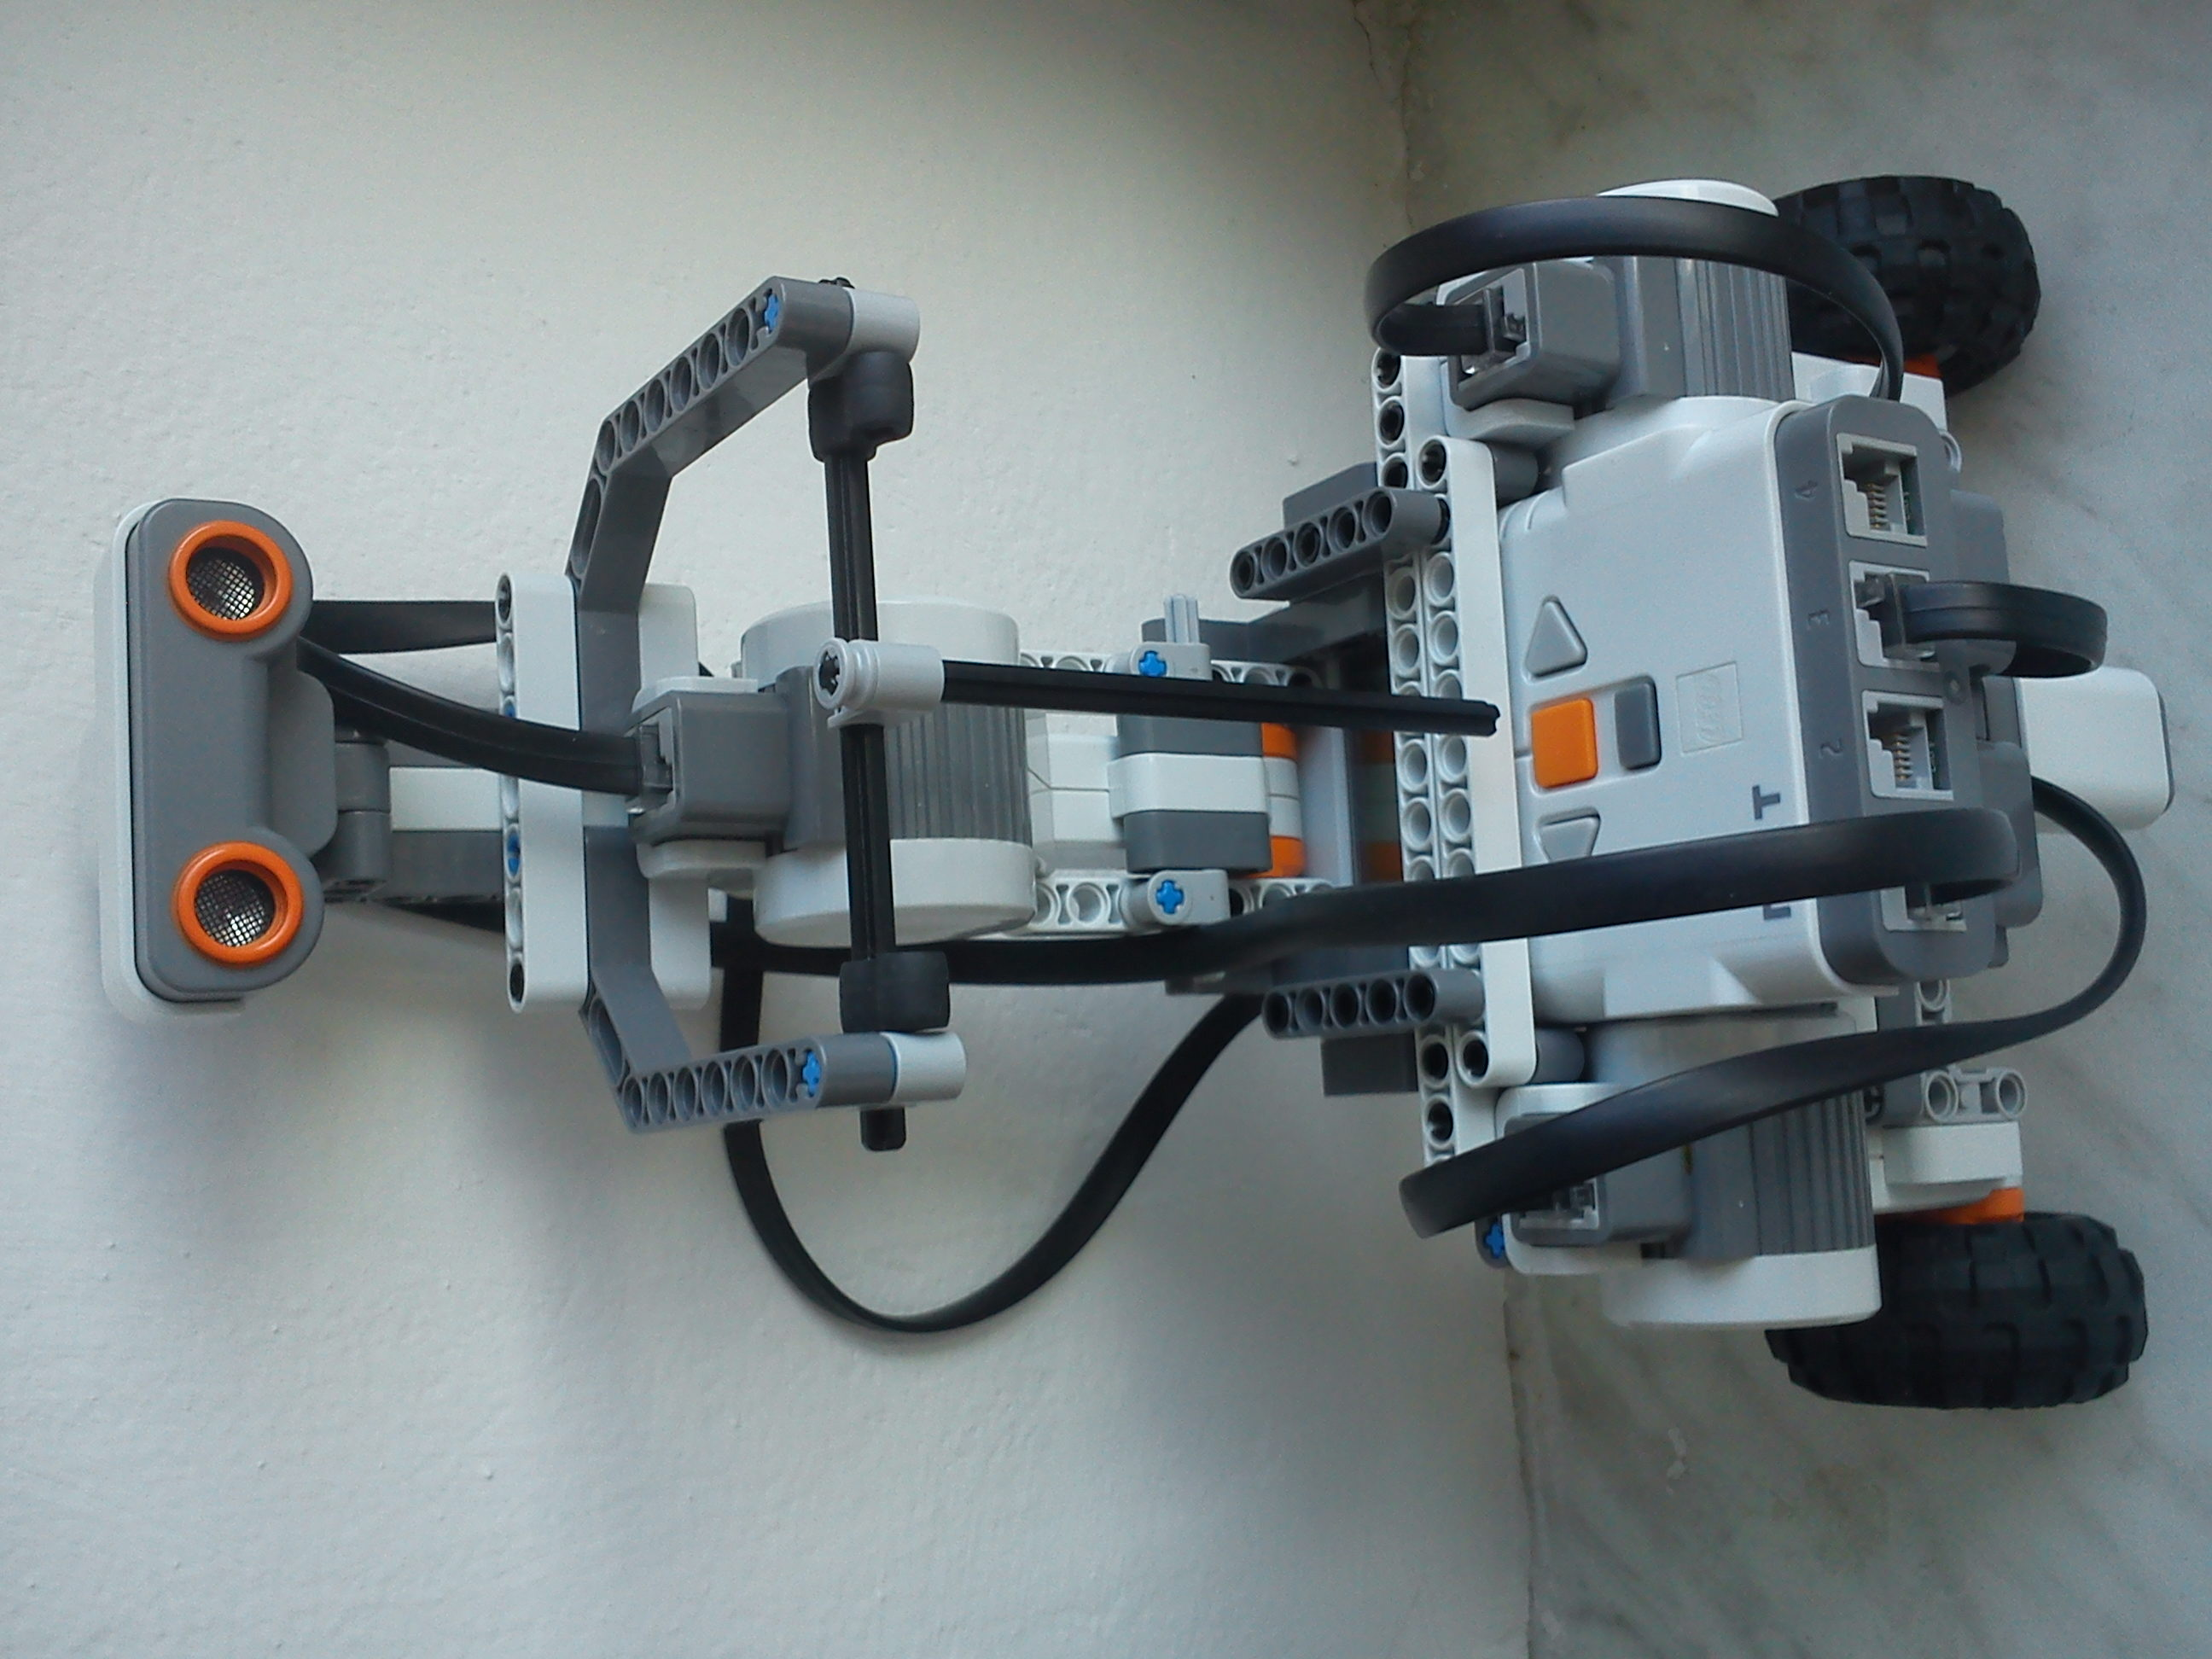
\includegraphics[height=4cm, angle=270]{legway}
    \caption{Legway}
    \label{fig:legway}
\end{figure}

\end{frame}

\section{Controller}

\begin{frame}
\frametitle{PID - feedback loop}

\begin{figure}[h]
    \centering
    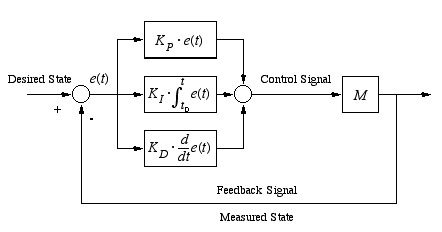
\includegraphics[width=8cm]{pid}
    \caption{PID controller in controll loop}
    \label{fig:pid}
\end{figure}

\end{frame}

\begin{frame}
\frametitle{PID - equations}

\begin{itemize}
    \item PID:
        $$u(t) = K \left( e(t) + \frac{1}{T_i} \int_0^t e(\tau)d\tau + T_d
        \frac{de(t)}{dt} \right)$$
    \item Parallel version of PID equation:
        $$u(t) =  K_pe(t) + K_i \int_0^t e(\tau)d\tau + K_d \frac{de(t)}{dt}$$
    \pause \item Constants:
    \begin{itemize}
        \item $K_p$ - proportional gain
        \item $K_i$ - integral gain
        \item $K_d$ - derivative gain
    \end{itemize}
\end{itemize}

\end{frame}

\begin{frame}
\frametitle{PID - discrete form}

\begin{itemize}
    \item Laplace transform - Laplace form:
        $$G(s) = K_p + \frac{K_i}{s} + sK_d$$
    \pause \item Z-transform - Difference form:
        $$u[k] = u[k-1] + K_1e[k]+K_2e[k-1]+K_3e[k-2]$$

    \item Constants:
        \begin{eqnarray*}
            K_1 &=& K_p + K_i + K_d \\
            K_2 &=& -K_p-2K_d \\
            K_3 &=& K_d
        \end{eqnarray*}

\end{itemize}

\end{frame}

\section{Remote control}
\frame{
	\frametitle{Remote control}
	\begin{itemize}
		\item User can just control speed
		\item Application for Android written in Scala
		\item Communication via Bluetooth
			\begin{itemize}
				\item on top of NXT-specific protocol
			\end{itemize}
		\item Realtime protocol design
	\end{itemize}
}

\frame{
	\frametitle{Security and safety challenges}
	\begin{itemize}
		\item Spoofed commands
		\item Delays
			\begin{itemize}
				\item Natural
				\item Caused by an adversary
			\end{itemize}
		\item Lost connection
	\end{itemize}
}

\frame{
	\frametitle{Security and safety solutions}
	\begin{itemize}
		\item Authorization hopefully solved on the RFCOMM layer
		\item Delays and lost connection: \texttt{validUntil}
		\item Remaining challenge: time sync
	\end{itemize}
}

\frame{
	\frametitle{Syncing the time}
	\begin{itemize}
		\item No time dilation assumption
		\item No global time
		\item Syncing approaches:
			\begin{enumerate}[a]
				\item Negligible delays assumption
				\item Confirmation of message delivery
				\item Confirmation of processed message (ideal)
			\end{enumerate}

	\end{itemize}
}


\begin{frame}
    \Huge{\centerline{Thank you for your attention.}}
\end{frame}

%----------------------------------------------------------------------------------------

\end{document}
